\documentclass[11pt,a4paper,DIV=12]{scrartcl}
\PassOptionsToPackage{dvipsnames}{xcolor}
\usepackage{multicol}
\makeatletter
\def\input@path{{../../../}}
\makeatother

\usepackage[sexy]{evan}

\makeatletter
\newtheoremstyle{problemstyle}
  {8pt} 
  {8pt} 
  {\normalfont} 
  {} 
  {\color{blue!40!black}\bfseries} 
  {} 
  {0.5em} 
  {\thmnumber{#2}.\thmnote{ (\small #3)}} 

\let\problem\@undefined
\let\endproblem\@undefined
\let\c@problem\@undefined
\let\theproblem\@undefined
\makeatother

\makeatletter
\newtheoremstyle{answerstyle}
  {8pt} 
  {8pt} 
  {\normalfont} 
  {}
  {\color{blue!40!black}\bfseries} 
  {} 
  {\newline} 
  {\thmnumber{#2}. \thmnote{\fbox{\bfseries #3}}} 

\let\answer\@undefined
\let\endanswer\@undefined
\let\c@answer\@undefined
\let\theanswer\@undefined
\makeatother

\newcommand\answerbox{%%
\vspace*{0.5cm}%
\noindent\textbf{\textsf{Jawab}}: \fbox{\rule{14cm}{0pt}\rule[-0.2ex]{0pt}{1.9ex}}}

\theoremstyle{problemstyle}
\newtheorem{problem}{}
\theoremstyle{answerstyle}
\newtheorem{answer}{}

\newenvironment{choices}[1][5]{%
\raggedcolumns
  \begin{multicols}{#1}%
  \begin{enumerate}[label=(\Alph*)]%
}{%
  \end{enumerate}%
  \end{multicols}%
}

\begin{document}
\title{Tryout 3 Pembinaan OSK Matematika}
\author{MAN 1 Pasuruan}
\date{Juni 2025}
\maketitle
\noindent\textbf{Petunjuk pengerjaan:}
\begin{itemize}
  \item Waktu pengerjaan adalah 120 menit.
  \item Terdapat 20 soal yang terdiri dari 10 soal pilihan ganda dan 10 soal kemampuan isian singkat.
  \item Nilai soal pilihan ganda adalah {\color{green!70!black}$B=+1$}, {\color{red}$S=0$}, $K=0$.
  \item Nilai soal isian singkat adalah {\color{green!70!black}$B=+4$}, {\color{red}$S=0$}, $K=0$.
  \item Gunakan bolpoin untuk menulis jawaban, dan coretlah jawaban yang salah.
\end{itemize}

\section*{Pilihan Ganda}
\begin{problem}
  Setiap persegi pada kotak berukuran $3 \times 3$ diwarnai merah, putih, biru, atau hijau sedemikian rupa sehingga setiap persegi berukuran $2 \times 2$ berisi satu persegi dari setiap warna. Salah satu pewarnaan tersebut ditunjukkan pada gambar di bawah. Berapa banyak pewarnaan berbeda yang mungkin terjadi?
  \begin{center}
    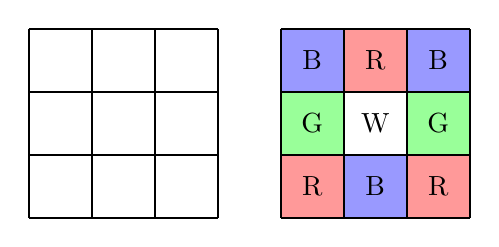
\begin{tikzpicture}[scale=0.8, thick]
      \fill[blue!40]  (0,2) rectangle (1,3);
      \fill[red!40]   (1,2) rectangle (2,3);
      \fill[blue!40]  (2,2) rectangle (3,3);

      \fill[green!40] (0,1) rectangle (1,2);
      \fill[white]    (1,1) rectangle (2,2);
      \fill[green!40] (2,1) rectangle (3,2);

      \fill[red!40]   (0,0) rectangle (1,1);
      \fill[blue!40]  (1,0) rectangle (2,1);
      \fill[red!40]   (2,0) rectangle (3,1);

      \draw (-4,0) grid (-1,3);
      \draw (0,0) grid (3,3);

      \node at (0.5, 2.5) {B}; \node at (1.5, 2.5) {R}; \node at (2.5, 2.5) {B};
      \node at (0.5, 1.5) {G}; \node at (1.5, 1.5) {W}; \node at (2.5, 1.5) {G};
      \node at (0.5, 0.5) {R}; \node at (1.5, 0.5) {B}; \node at (2.5, 0.5) {R};
    \end{tikzpicture}
  \end{center}

  \begin{choices}
    \item $24$
    \item $48$
    \item $60$
    \item $72$
    \item $96$
  \end{choices}
  %KJ : D
\end{problem}

\begin{problem}
  Suzanne pergi ke bank dan menarik uang sebesar $\$800$. Teller memberikan jumlah tersebut menggunakan lembaran pecahan $\$20$, $\$50$, dan $\$100$, dengan setidaknya satu lembar dari setiap pecahan. Berapa banyak koleksi lembaran berbeda yang bisa diterima oleh Suzanne?

  \begin{choices}
    \item $45$
    \item $21$
    \item $36$
    \item $28$
    \item $32$
  \end{choices}
  %KJ : B
\end{problem}

\begin{problem}
  Masing-masing dari $2023$ bola dimasukkan secara acak ke dalam salah satu dari $3$ keranjang. Manakah dari berikut ini yang paling mendekati peluang bahwa setiap keranjang akan berisi jumlah bola yang ganjil?
  \begin{choices}
    \item $\frac{2}{3}$
    \item $\frac{3}{10}$
    \item $\frac{1}{2}$
    \item $\frac{1}{3}$
    \item $\frac{1}{4}$
  \end{choices}
  %KJ : E
\end{problem}

\begin{problem}
  Pablo akan menghias masing-masing dari $6$ bola putih yang identik dengan pola bergaris atau berbintik, menggunakan cat merah atau biru. Ia akan menentukan warna dan pola untuk setiap bola dengan melempar koin yang adil untuk setiap dari $12$ keputusannya. Setelah cat mengering, ia menempatkan $6$ bola tersebut ke dalam sebuah guci. Frida akan memilih secara acak satu bola dari guci tersebut dan mencatat warna serta polanya. Kejadian "bola yang dipilih Frida berwarna merah" dan "bola yang dipilih Frida berpola bergaris" mungkin saling bebas atau tidak, bergantung pada hasil lemparan koin Pablo. Peluang bahwa kedua kejadian ini saling bebas dapat ditulis sebagai $\frac{m}{n}$, di mana $m$ dan $n$ adalah bilangan bulat positif yang saling prima. Berapakah nilai $m$? (\emph{Ingat bahwa dua kejadian $A$ dan $B$ saling bebas jika $P(A \cap B) = P(A) \cdot P(B)$})
  \begin{choices}
    \item $243$
    \item $245$
    \item $247$
    \item $249$
    \item $251$
  \end{choices}
  %KJ : A
\end{problem}

\begin{problem}
  Berapa banyak tripel terurut $(x, y, z)$ dari bilangan bulat positif berbeda yang kurang dari atau sama dengan $8$ yang memenuhi $xy > z$, $xz > y$, dan $yz > x$?

  \begin{choices}
    \item $36$
    \item $84$
    \item $186$
    \item $336$
    \item $486$
  \end{choices}
  %KJ : C
\end{problem}

\begin{problem}
  Misalkan $P(x)=x^{2022}+x^{1011}+1$. Manakah dari polinomial berikut yang merupakan faktor dari $P(x)$?

  \begin{choices}
    \item $x^2-x+1$
    \item $x^2+x+1$
    \item $x^4+1$
    \item $x^6-x^3+1$
    \item $x^6+x^3+1$
  \end{choices}
  %KJ : E
\end{problem}

\begin{problem}
  Berapa banyak pasangan terurut $(b,c)$ dari bilangan bulat positif sehingga baik $x^2+bx+c=0$ maupun $x^2+cx+b=0$ tidak memiliki dua akar real berbeda?

  \begin{choices}
    \item $4$
    \item $6$
    \item $8$
    \item $12$
    \item $16$
  \end{choices}
  %KJ : B
\end{problem}

\begin{problem}
  Manakah dari pilihan berikut yang ekuivalen dengan
  \[
    (2+3)(2^2+3^2)(2^4+3^4)(2^8+3^8)(2^{16}+3^{16})(2^{32}+3^{32})(2^{64}+3^{64})?
  \]
  \begin{choices}[2]
    \item $3^{127}+2^{127}$
    \item $3^{127}+2^{127}+2\cdot 3^{63}+3\cdot 2^{63}$
    \item $3^{128}-2^{128}$
    \item $3^{128}+2^{128}$
    \item $5^{127}$
  \end{choices}
  %KJ : C
\end{problem}

\begin{problem}
  Untuk $x\geq 0$, nilai terkecil dari $\dfrac{4x^2+8x+13}{6+6x}$ adalah $\ldots$

  \begin{choices}
    \item $0$
    \item $1$
    \item $2$
    \item $4$
    \item $5$
  \end{choices}
  %KJ : C
\end{problem}

\begin{problem}
  Tentukan nilai maksimum dari $a+2b+3c$ jika $a^2+b^2+c^2=4$ dengan $a,b,c\in\mathbb{R}$.

  \begin{choices}
    \item $2\sqrt{6}$
    \item $2\sqrt{10}$
    \item $2\sqrt{14}$
    \item $4\sqrt{3}$
    \item $4\sqrt{5}$
  \end{choices}
  %KJ : C
\end{problem}

\section*{Isian Singkat}
\begin{problem}
  Henry dan Charles memiliki $2021$ donat di dalam kulkas mereka. Selain itu, Henry memiliki dua belas keranjang dan Charles memiliki $m$ keranjang, dengan $m$ adalah suatu bilangan asli. Tentukan banyak bilangan asli $m$ yang memenuhi sehingga Henry dapat mengambil beberapa donat dari dalam kulkas tersebut dan menaruhnya ke dalam semua keranjangnya dengan sama rata, kemudian Charles dapat menaruh semua donat yang tersisa ke dalam semua keranjangnya dengan sama rata juga.\\
  \textit{Catatan: Semua keranjang milik Henry maupun Charles harus terisi setidaknya satu donat.}

  \answerbox
  %KJ : 241
\end{problem}

\begin{problem}
  Budi menulis semua permutasi dari angka $1,2,\dots,9$. Tentukan banyak angka yang ditulis Budi yang tidak memuat angka $45$, $56$ atau $849$ secara berurutan.

  \answerbox
  %KJ : 282960
\end{problem}

\begin{problem}
  Banyaknya tripel bilangan bulat $(x,y,z)$ dengan $0 \le x \le y \le z$ yang memenuhi persamaan $x + y + z = 32$ adalah \dots

  \answerbox
  %KJ : 102
\end{problem}

\begin{problem}
  Ani dan Banu bermain dadu enam sisi. Jika dadu yang keluar bernilai genap, maka Ani mendapatkan skor $1$ sedangkan jika dadu yang keluar bernilai ganjil, maka Banu yang mendapatkan skor $1$. Pemenang dari permainan ini adalah orang pertama yang mendapatkan skor total $5$. Setelah dilakukan pelemparan dadu sebanyak $5$ kali, Ani mendapat skor $4$ dan Banu mendapatkan skor $1$. Peluang Ani memenangkan permainan ini adalah \dots

  \answerbox
  %KJ : 15/16
\end{problem}

\begin{problem}
  Banyaknya bilangan delapan digit yang setiap digitnya adalah $1$ atau $2$ tetapi tidak memuat tiga digit $1$ berurutan adalah \dots

  \answerbox
  %KJ : 149
\end{problem}

\begin{problem}
  Diberikan bilangan real $a$ dan $b$. Nilai minimum dari
  $
    5a^2 + 18b^2 + 12ab - 10a + 60b + 150
  $
  adalah \dots

  \answerbox
  %KJ : 25
\end{problem}

\begin{problem}
  Diketahui bilangan real $a, b, c$ memenuhi persamaan
  \[
    a^2 + b^2 + c^2 = 2a + 4b + 6c
  \]
  Jika nilai terbesar yang mungkin dari $a + b + c$ dapat dinyatakan dalam bentuk $x + \sqrt{y}$ dengan $x$ dan $y$ merupakan bilangan asli, maka nilai dari $x + y$ adalah \dots

  \answerbox
  %KJ : 48
\end{problem}

\begin{problem}
  Misalkan $a,b,c\in\mathbb{R}^+$ dengan $a+b+c=1$. Tentukan nilai minimum dari
  $
    a^2+b^2+c^2
  $.

  \answerbox
  %KJ : 1/3
\end{problem}

\begin{problem}
  Tentukan nilai maksimum dari
  $
    \sqrt{x}+\sqrt{3x-2}+\sqrt{5-4x}
  $
  dengan $x$ bilangan real.

  \answerbox
  %KJ : 3
\end{problem}

\begin{problem}
  Pada sebarang segitiga dengan semi-keliling $s$ dan jari-jari lingkaran dalam $r$. Tentukan nilai minimum dari $\dfrac{s}{r}$.
  \textit{(Hint: rumus luas segitiga adalah $A = r \cdot s$)}

  \answerbox
  %KJ : 3\sqrt{3}
\end{problem}

\end{document}